\documentclass[xcolor=table, aspectratio=43]{beamer}
%\usepackage[english]{babel}

%Cargar paquetes
\usepackage[utf8]{inputenc}%Permite usar acentos
\usepackage[spanish]{babel}%Configura el idioma por defecto a español
\usepackage{amsmath}%Introduce términos matemáticos
\usepackage{graphicx}%Permite introducir figuras
\usepackage[options]{natbib}%Bibliografía con estilos %No funcionan estilos en Beamer
\newcommand{\grad}{\hspace{-2mm}$\phantom{a}^{\circ}$}

\usepackage{amsthm}
\usepackage{mathtools}
\usepackage{physics}
\usepackage{calligra}
\usepackage{csquotes}
\usepackage{tensor}
\usepackage[thicklines]{cancel}
\usepackage{tcolorbox}
\usepackage{pstricks}
\usepackage[backend=biber, bibstyle=nature, sorting=nty, citestyle=numeric-comp]{biblatex} %Custom bibliography
    \addbibresource{bib.bib} %Load references


\DeclareMathAlphabet{\mathcalligra}{T1}{calligra}{m}{n}
\DeclareFontShape{T1}{calligra}{m}{n}{<->s*[2.2]callig15}{}
\newcommand{\scriptr}{\mathcalligra{r}\,}
\newcommand{\boldscriptr}{\pmb{\mathcalligra{r}}\,}
\def\rc{\scriptr}
\def\brc{\boldscriptr}
\def\hrc{\hat\brc}
\newcommand{\ie}{\emph{i.e.}} %id est
\newcommand{\eg}{\emph{e.g.}} %exempli gratia
\newcommand{\rtd}[1]{\ensuremath{\left\lfloor #1 \right\rfloor}}
\newcommand{\dirac}[1]{\ensuremath{\delta \left( #1 \right)}}
\newcommand{\diract}[1]{\ensuremath{\delta^3 \left( #1 \right)}}
\newcommand{\e}{\ensuremath{\epsilon_0}}
\newcommand{\m}{\ensuremath{\mu_0}}
\newcommand{\V}{\ensuremath{\mathcal{V}}}
\newcommand{\prnt}[1]{\ensuremath{\left(#1\right)}} %parentheses
\newcommand{\colch}[1]{\ensuremath{\left[#1\right]}} %square brackets
\newcommand{\chave}[1]{\ensuremath{\left\{#1\right\}}}  %curly brackets

\useoutertheme{infolines}
\useinnertheme{rectangles}
\usefonttheme{professionalfonts}


\definecolor{orange}{HTML}{f28165}
\definecolor{gray}{HTML}{303030}
\definecolor{yellow}{HTML}{f0be52}
\definecolor{lightorange}{HTML}{f19e58}

\renewcommand{\CancelColor}{\color{orange}}

\makeatletter
\newcommand{\mybox}[1]{%
  \setbox0=\hbox{#1}%
  \setlength{\@tempdima}{\dimexpr\wd0+13pt}%
  \begin{tcolorbox}[colback=orange,colframe=orange,boxrule=0.5pt,arc=4pt,
      left=6pt,right=6pt,top=6pt,bottom=6pt,boxsep=0pt,width=\@tempdima]
    \textcolor{white}{#1}
  \end{tcolorbox}
}
\makeatother

\usecolortheme[named=orange]{structure}
\usecolortheme{sidebartab}
\usecolortheme{orchid}
\usecolortheme{whale}
\setbeamercolor{alerted text}{fg=yellow}
\setbeamercolor{block title alerted}{bg=alerted text.fg!90!black}
\setbeamercolor{block title example}{bg=lightorange!60!black}
\setbeamercolor{background canvas}{bg=gray}
\setbeamercolor{normal text}{bg=gray,fg=white}

\setbeamertemplate{footline}
        {
      \leavevmode%
      \hbox{%
      \begin{beamercolorbox}[wd=.333333\paperwidth,ht=2.25ex,dp=1ex,center]{author in head/foot}%
        \usebeamerfont{author in head/foot}\insertshortauthor~~(\insertshortinstitute)
      \end{beamercolorbox}%
      \begin{beamercolorbox}[wd=.333333\paperwidth,ht=2.25ex,dp=1ex,center]{title in head/foot}%
        \usebeamerfont{title in head/foot}\insertshorttitle
      \end{beamercolorbox}%
      \begin{beamercolorbox}[wd=.333333\paperwidth,ht=2.25ex,dp=1ex,center]{date in head/foot}%
        \usebeamerfont{page number in head/foot}\insertframenumber/\inserttotalframenumber%\hspace*{2em}

    %#turning the next line into a comment, erases the frame numbers
        %\insertframenumber{} / \inserttotalframenumber\hspace*{2ex} 

      \end{beamercolorbox}}%
      \vskip0pt%
    }


\setbeamertemplate{blocks}[rectangle]
\setbeamercovered{dynamic}

\setbeamertemplate{section page}
{
	\begin{centering}
		\begin{beamercolorbox}[sep=27pt,center]{part title}
			\usebeamerfont{section title}\insertsection\par
			\usebeamerfont{subsection title}\insertsubsection\par
		\end{beamercolorbox}
	\end{centering}
}

%\setbeamertemplate{subsection page}
%{
%	\begin{centering}
%		\begin{beamercolorbox}[sep=12pt,center]{part title}
%			\usebeamerfont{subsection title}\insertsubsection\par
%		\end{beamercolorbox}
%	\end{centering}
%}

\newcommand{\hlight}[1]{\colorbox{violet!50}{#1}}
\newcommand{\hlighta}[1]{\colorbox{red!50}{#1}}
\title{Análisis de entrada} %->->->->-> Check hyperref title <-<-<-<-<-
%\subtitle{And Some Things About It}
\author[C.J. Uribe-Martes]{Carlos Javier Uribe Martes}
\institute[CUC]{
    Ingeniería Industrial%
    \\%
    Universidad de la Costa%
} %You can change the Institution if you are from somewhere else
\date{Marzo 24, 2020}
%\logo{\includegraphics[width= 0.2\textwidth]{images/a-logo.png}}

\begin{document}
    
    \frame{\titlepage}
    
    \begin{frame}{Contenido}
        \tableofcontents
    \end{frame}
    
    \section{Introducción}

\begin{frame}{Análisis de entrada}
    \begin{itemize}
        \item Para llevar a cabo una simulación utilizando entradas aleatorias debemos especificar sus distribuciones de probabilidad \cite{LK}.
        \item Seleccionar distribuciones de probabilidad adecuadas es una tarea importante y que requiere tiempo y buenos análisis estadísticos. \cite{BCN}.
        %\item En esta parte nos centraremos en cómo el analista especifica estas distribuciones de probabilidad de entrada.
    \end{itemize}
\end{frame}

\begin{frame}{Análisis de entrada}

    La metodología para conducir un Análisis de entrada incluye los siguientes pasos:
    \begin{enumerate}
        \item Recolección de datos.
        \item Análisis de datos.
        \item Modelado de datos.
        \item Pruebas de bondad de ajuste.
    \end{enumerate}
\end{frame}
    
    \section{Recolección de datos}

\begin{frame}{Recolección de datos}
    \begin{itemize}
        \item Aún teniendo un modelo válido, si los datos se recogen de una manera inadecuada, o son analizados incorrectamente, los resultados del modelo serán erróneos y pueden conducir a malas decisiones.
        \item Hay riesgos derivados de la escasez de datos disponibles, o de datos irrelevantes, desactualizados o simplemente erróneos.
    \end{itemize}
\end{frame}


\begin{frame}{Recolección de datos}
    \begin{itemize}
        \item Algunas sugerencias para la recolección de datos son:
    \begin{itemize}
        \item Planeación: observación del sistema actual y situaciones atípicas.
        \item Análisis de los datos a medida que son recolectados.
        \item Verificar homogeneidad en los diferentes grupos de datos.
        \item Revisar la relación entre variables.
        \item Revisar autocorrelación.
        \item Diferenciar claramente entre datos de entrada y de salida.
    \end{itemize}
    \end{itemize}
\end{frame}


\begin{frame}{Modelos de entrada sin datos}
    \begin{itemize}
        \item Si el sistema a modelar No existe, el analista debe confiar en datos más vagos, que pueden incluir:
        \begin{enumerate}
            \item Experiencias previas.
            \item Opinión de expertos.
            \item Intuición.
            \item Conjeturas a partir de las limitaciones físicas, datos de ingeniería, estándares o la naturaleza del proceso.
        \end{enumerate}
    \end{itemize}
\end{frame}

\begin{frame}{Modelos de entrada sin datos}
    \begin{itemize}
        \item En muchas aplicaciones de la vida real, se utilizan heurísticas como:
    \begin{itemize}
        \item Variables aleatorias con poca variabilidad se simplifican y modelan como deterministas.
        \item Para distribuciones desconocidas se postulan forma funcionales particulares que incorporen cualquier información disponible (Triangular, Uniforme). 
        \item La experiencia a veces puede proporcionar información sobre la forma funcional de las distribuciones.
    \end{itemize}
    \end{itemize}
\end{frame}

\begin{frame}{Modelos de entrada con datos}
    \begin{itemize}
    \item Si el sistema a modelar ya existe, entonces puede proporcionar los datos empíricos necesarios a partir de mediciones en campo.
    \end{itemize}
\end{frame}

\begin{frame}{¿Qué datos se requieren tomar?}
    \begin{itemize}
        \item Dentro de los datos de entrada a recolectar se requieren aquellos relacionados con tiempos entre llegadas, tiempos de servicio, tiempo a la falla de máquinas/recursos, duración de las fallas, tiempos de desplazamiento, probabilidades de tener ciertos valores de atributos (tipos de cliente, cantidad de demanda).
        \item La recolección de datos de las medidas de desempeño del sistema en estudio también es esencial para la validación del modelo.
        %\item Dichas mediciones empíricas deben recolectarse de forma rutinaria siempre que sea posible con miras a la validación futura.
    \end{itemize}
\end{frame}

\begin{frame}{¿Cuántos datos se requiere tomar?}
    \begin{itemize}
        \item Si $\bar{x}$ es un estimador de $\mu$, se puede tener un $100\left(1-\alpha\right)$\% de confianza de que el error no excederá una cantidad específica $e$ cuando el tamaño de muestra sea:
        \[n=\left(\dfrac{z_{\alpha/2}\times \sigma}{e}\right)^2\]
    \end{itemize}
    \begin{figure}
        \centering
        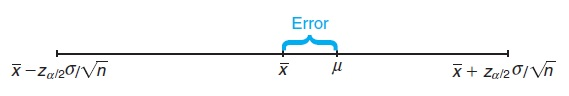
\includegraphics[width=8cm]{images/error_x.jpg}
        %\caption{Caption}
        %\label{fig:my_label}
    \end{figure}
\end{frame}

\begin{frame}{¿Cuántos datos se requiere tomar?}
    \begin{itemize}
        \item Si $\hat{p}$ es un estimador de $p$, se puede tener un $100\left(1-\alpha\right)$\% de confianza de que el error no excederá una cantidad específica $e$ cuando el tamaño de muestra sea:
        \[n=\left(\dfrac{z^2_{\alpha/2}\times \hat{p} \times \hat{q}}{e^2}\right)\]
    \end{itemize}
    \begin{figure}
        \centering
        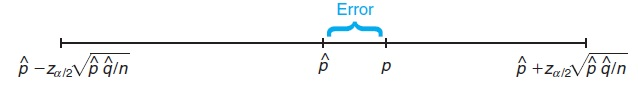
\includegraphics[width=8cm]{images/error_p.jpg}
        %\caption{Caption}
        %\label{fig:my_label}
    \end{figure}
\end{frame}
    
    \section{Análisis de datos}

\begin{frame}{Análisis de datos}
    \begin{itemize}
        \item El análisis de datos implica el cálculo de varias estadísticas a partir de los datos recopilados:
    \begin{itemize}
        \item Estadísticas relacionadas con los momentos (media, desviación estándar, coeficiente de variación, etc.).
        \item Estadísticas relacionadas con distribuciones (histogramas, q-q plot, p-p plot).
        \item Estadísticas relacionadas con la dependencia temporal (autocorrelaciones dentro de una serie temporal empírica o correlaciones cruzadas entre dos o más series temporales distintas).
    \end{itemize}
    \end{itemize}
\end{frame}

\begin{frame}{Estimación de media y varianza muestral}
    \begin{itemize}
        \item Si las observaciones en una muestra de tamaño $n$ son $x_1,x_2,\dots,x_n$, la media muestral y la varianza muestral están dadas por:
            \begin{equation*}
                \bar{X}=\frac{\sum\limits_{i=1}^{n}x_i}{n}
            \end{equation*}
            \begin{equation*}
                S^2=\frac{\sum\limits_{i=1}^{n}{x_i^2}-n\bar{X}^2}{n-1}
            \end{equation*}
        %\item 
    \end{itemize}
\end{frame}

\begin{frame}{Estimadores de estadísticas para distribuciones comunes}

    \begin{table}[]
    \begin{tabular}{|lll|}
    \hline
    \rowcolor[HTML]{DAE8FC} 
    \multicolumn{1}{|l|}{\cellcolor[HTML]{79403D}\textbf{Distribución}} & \multicolumn{1}{l|}{\cellcolor[HTML]{79403D}\textbf{Parámetros}} & \multicolumn{1}{l|}{\cellcolor[HTML]{79403D}\textbf{Estimadores}} \\ \hline
    \textit{Poisson} & $\alpha$ & $\hat{\alpha}=\bar{X}$ \\ \hline
    \textit{Exponencial} & $\lambda$ & $\hat{\lambda}=\frac{1}{\bar{X}}$ \\ \hline
    \textit{Gamma} & $\beta,\theta$ & \begin{tabular}[c]{@{}l@{}}$\hat{\beta}$ ver Tabla estimadores \\ de máxima verosimilitud\\ $\hat{\theta}=\frac{1}{\bar{X}}$\end{tabular} \\ \hline
    \textit{Normal} & $\mu,\sigma^2$ & \begin{tabular}[c]{@{}l@{}}$\hat{\mu}=\bar{X}$\\ $\hat{\sigma}^2=S^2$\end{tabular} \\ \hline
    \textit{Lognormal} & $\mu,\sigma^2$ & \begin{tabular}[c]{@{}l@{}}$\hat{\mu}=\bar{X}$ luego \\ de sacar $\ln$ a los datos\\ $\hat{\sigma}^2=S^2$ luego \\ de sacar $\ln$ a los datos\end{tabular} \\ \hline
    \end{tabular}
    \end{table}
\end{frame}

\begin{frame}{Histogramas}
    \begin{itemize}
        \item Son útiles para la identificación de la forma de una distribución.
        \begin{itemize}
            \item El número de clases, $k$ depende del número de observaciones $n$ y de la dispersión de los datos. Puede usarse:
                \begin{equation*}
                    k=\sqrt{n}
                \end{equation*}
                o
                \begin{equation*}
                    k=1+3.322 \log_{10}{n}
                \end{equation*}
            \item Si los intervalos son muy anchos el histograma no mostrará  un comportamiento claramente.
        \end{itemize}
        %\item Un histograma da una idea, pero no debe usarse como única herramienta de identificación.
    \end{itemize}
\end{frame}

\begin{frame}{Q-Q plot}
    \begin{itemize}
        \item Sea $X$ una variable aleatoria con función acumulada de probabilidad $F_x(X)$, entonces el $q$-cuantil de $X$ es aquel valor $\gamma$ tal que $F_x(X)=P(X\leq \gamma)=q$. Si $F$ tiene inversa entonces $\gamma = F^{-1}(q)$.
        \item Para realizar una Q-Q plot se emplea el siguiente algoritmo:
        \begin{enumerate}
            \item Tomar una muestra de los datos $x_i,~ i=1,2,\dots, n$ y ordenarlos para obtener $y_j,~j=1,2,\dots,n$.
            \item $y_j$ es una estimación del $\left[\frac{j-\left(\frac{1}{2}\right)}{n}\right]$ cuantil de $X$. Esto es $y_j \sim F^{-1}\left[\frac{j-\left(\frac{1}{2}\right)}{n}\right]$.
            \item Graficar $y_j$ vs $F^{-1}\left[\frac{j-\left(\frac{1}{2}\right)}{n}\right]$
            \item Si los datos corresponden a la distribución que se está probando, la gráfica debe ser aproximadamente una línea recta.
        \end{enumerate}
    \end{itemize}
\end{frame}

\begin{frame}{Q-Q plot}
    Algunas consideraciones al realizar una Q-Q plot:
    \begin{itemize}
        \item Nunca es realmente una línea recta.
        \item Un punto encima de la línea será probablemente seguido por otro.
        \item La variación en los extremos es más grande. La linealidad en el centro es más importante que la linealidad en los extremos.
    \end{itemize}
\end{frame}

\begin{frame}{P-P plot}
    \begin{itemize}
        \item Utiliza la probabilidad acumulada para verificar si una muestra de datos sigue una distribución de probabilidad en particular, mediante el siguiente algoritmo:
        \begin{enumerate}
        \item Tomar una muestra de los datos $x_i,~i=1,2,\dots,n$ y ordenarlos para obtener $y_j,~j=1,2,\dots,n$.
        \item Para cada valor de la muestra calcular $q_j=\left[\frac{j-\left(\frac{1}{2}\right)}{n}\right]$.
        \item Graficar $q_j$ vs $F_x(y_j)$.
        \item Si los datos corrsponden a la distribución que se está probando, la gráfica debe ser aproximadamente un línea recta.
    \end{enumerate}
    \end{itemize}
\end{frame}

\begin{frame}{Diferencias entre Q-Q plot y P-P plot}
    \begin{itemize}
        \item Un P-P plot compara la función de probabilidad acumulada de una muestra de datos con una función de probabilidad específica $F(\cdot)$, mientras que un Q-Q plot compara los cuantiles estimados dada una función de probabilidad con una muestra de datos.
        \item El rango de un P-P plot siempre es entre 0 y 1, el rango del Q-Q plot depende del rango de la función de probabilidad y de los datos observados.
        \item Un Q-Q plot amplifica las diferencias existentes en las colas del gráfico, mientras que un P-P plot amplifica las diferencias en el centro.
    \end{itemize}
\end{frame}

    
    \section{Modelado de datos}

\begin{frame}{Modelado de datos}
    \begin{itemize}
        \item En esta etapa, un modelo probabilístico es ajustado a las series de tiempo empíricas recolectadas.
        \item Dependiendo del tipo de datos de series de tiempo que se van a modelar, esta etapa se puede clasificar en dos categorías:
        \begin{enumerate}
            \item Las observaciones independientes se modelan como una secuencia de variables aleatorias iid. En este caso, se busca identificar (ajustar) una distribución y sus parámetros a los datos empíricos.
            \item Las observaciones dependientes se modelan como procesos aleatorios con dependencia temporal. En este caso, se requiere identificar (ajustar) una ley de probabilidad a los datos empíricos.
        \end{enumerate}
    \end{itemize}
\end{frame}

\begin{frame}{Identificación de distribuciones de probabilidad}
    \begin{itemize}
        \item Existen literalmente cientos de distribuciones de probabilidad.
        \item Algunas distribuciones aparecen muy a menudo en estudios de simulación:
        \begin{itemize}
            \item Binomial, Poisson, Normal, Lognormal, Exponencial, Gamma, Beta, Erlang, Weibull, Uniforme, Triangular, ...
        \end{itemize}
    \end{itemize}
\end{frame}


    
    \section{Pruebas de bondad de ajuste}

\begin{frame}{Pruebas de bondad de ajuste}
    \begin{itemize}
        \item Las pruebas de bondad de ajuste son pruebas de hipótesis para verificar si los datos observados en una muestra aleatoria se ajustan con algún nivel de significancia a determinada distribución de probabilidad.
        \item Las hipótesis son:
        \begin{itemize}
            \item $H_0$: la variable aleatoria $X$ sigue una distribución asumida con los parámetros estimados.
            \item $H_1$: la variable aleatoria $X$ no sigue la distribución asumida.
        \end{itemize}
        \item Para realizar la prueba, se clasifican los datos observados en $k$ clases y se contabiliza el número de observaciones en cada clase, posteriormente se compara la frecuencia observada en cada clase con la frecuencia esperada en esa clase si la hipótesis nula es correcta.
    \end{itemize}
\end{frame}

\begin{frame}{Prueba chi-cuadrado}
    \begin{itemize}
        \item Considere $k>2$ el núméro de clases, $O_i$ la frecuencia observada en la clase $i$, $E_i$ la frecuencia esperada en la clase $i$ si $H_0$ es correcta.
        \item La prueba se basa en el estadístico de prueba chi-cuadrado:
        \[Y=\sum_{i=1}^{k}{\frac{\left(O_i-E_i\right)^2}{E_i}}\]
        \item El estadístico sigue una distribución chi-cuadrado con $k-r-1$ grados de libertad, donde $r$ es el número de parámetros estimados en $f_0(x)$ para encontrar $E_i$. 
    \end{itemize}
\end{frame}


\begin{frame}{Prueba chi-cuadrado}{Consideraciones}
    \begin{itemize}
        \item Si las diferencias $O_i-E_i$ son pequeñas, el valor del estadístico es pequeño, por el contrario si esas diferencias son grandes el valor del estadístico es grande.
        \item El tamaño de la muestra deberá ser moderadamente grande, pues si la muestra es muy pequeña no se podrá formar un número suficiente de clases y si la muestra es muy grande la prueba conducirá a rechazo casi con seguridad. 
        \item Se sugiere evitar tener clases con $E_i$ menores que 5, esto puede conseguirse combinando clases vecinas. Tenga en cuenta que para calcular los grados de libertad, $k$ es el número de clases efectivas.
    \end{itemize}
\end{frame}

\begin{frame}{Prueba chi-cuadrado}
    \begin{figure}
        \centering
        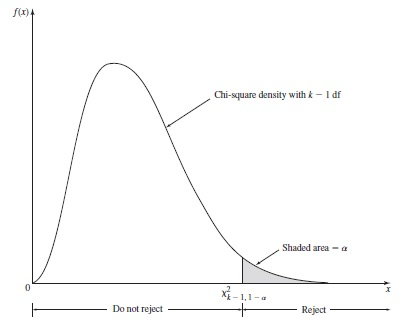
\includegraphics[width=8cm]{images/Chi-square.jpg}
        %\caption{Caption}
        \label{fig:chisquare}
    \end{figure}
\end{frame}
\begin{frame}{Prueba de Kolmogorov-Smirnov}
    \begin{itemize}
        \item Esta prueba formaliza la idea de una gráfica cuantil-cuantil y compara una función empírica de probabilidad con la función de la distribución hipotética. 
        \item No requiere de especificación de intervalos y es válida para cualquier tamaño de muestra.
    \end{itemize}
\end{frame}

\begin{frame}{Prueba de Kolmogorov-Smirnov}{Algoritmo}
    \begin{enumerate}
        \item Tomar una muestra de los datos $x_i,~i=1,2,\dots,n$ y ordenarlos para obtener $y_j,~j=1,2,\dots,n$.
        \item Estimar las diferencias por arriba y por abajo: $D^+=\max \left[ \frac{j}{n}-F(y_j)\right]$ y $D^-=\max \left[ F(y_j)-\frac{j-1}{n}\right]$. El estadístico de prueba está dado por: $D:\max \left[D^+,D^-\right]$
        \item Determine el valor crítico $D_\alpha$ para un nivel de significancia $\alpha$ y un tamaño de muestra $N$.
        \item Si el estadístico calculado es mayor que el valor crítico, entonces se rechaza la hipótesis nula. De lo contrario, se concluye que no hay evidencia estadística para recharzarla.
    \end{enumerate}
\end{frame}

\begin{frame}{Prueba de Kolmogorov-Smirnov}
\begin{figure}
    \centering
    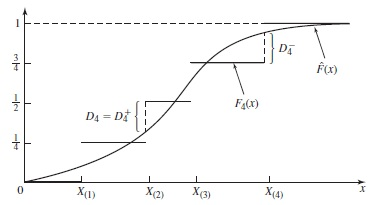
\includegraphics[width=8cm]{images/kolmogorov.jpg}
    %\caption{Caption}
    \label{fig:kolmogorov}
\end{figure}
\end{frame}

\begin{frame}{p-value}
    \begin{itemize}
        \item El p-value es el nivel de significancia en el que se rechazaría $H_0$ para el valor dado del estadístico de prueba. Por lo tanto, un p-value alto tiende a indicar un buen ajuste (tendríamos que aceptar una gran posibilidad de error para rechazar), mientras que un p-value pequeño sugiere un mal ajuste.
        \item El p-value se puede ver como una medida de ajuste, siendo mejores los valores más grandes. Regla de rechazo: si el p-value es menor que el nivel de significancia entonces se debe rechazar la hipótesis nula.
    \end{itemize}
\end{frame}
    
    %\section{Input Analyzer}

\begin{frame}{Input Analyzer}
    \begin{itemize}
        \item Input Analyzer es un complemento de Arena que puede emplearse para determinar la calidad del ajuste de datos de entrada a distintas funciones de distribución.
        \item Está disponible dentro de Arena en el menú Tools.
    \end{itemize}
\end{frame}

\begin{frame}{Preparación de archivos de datos}
    \begin{itemize}
        \item Se pueden crear en una hoja de cálculo o en un documento de texto.
        \begin{itemize}
            \item En una hoja de cálculo los datos se ingresan hacia abajo en una misma columna.
            \item En un documento de texto los datos deben separarse por: espacio, tabulaciones, guión corto.
        \end{itemize}
        \item Las extensiones del archivo pueden ser: .dst, .csv o .txt.
        \item Los datos no deben tener ningún tipo de encabezado.
        \item Se debe utilizar punto como separador decimal.
        \item No debe haber ningún tipo de caracter diferente a numéricos.
    \end{itemize}
\end{frame}

    \section*{Referencias} %You can remove this if you do not want to use it
        \begin{frame}{Referencias}
            \printbibliography
        \end{frame}
     
    \section{}   
        \begin{frame}{}
            \begin{figure}
                \centering
                
\includegraphics[width=6cm]{images/code.png}
                %\caption{Caption}
                %\label{fig:my_label}
            \end{figure}
        \end{frame}
      
\end{document}